\documentclass[UTF8,a4paper,12pt]{ctexart}  % Latex 去掉上面的语句,加上本语句
\usepackage{xeCJK}
\setCJKmainfont[BoldFont=AdobeHeitiStd-Regular]{AdobeSongStd-Light}
\setCJKfamilyfont{song}{AdobeSongStd-Light}
\setCJKfamilyfont{hei}{AdobeHeitiStd-Regular}
\setCJKfamilyfont{kai}{AdobeKaitiStd-Regular}
\setCJKfamilyfont{fs}{Sun Yat-sen Hsingshu}
% \setCJKmainfont[BoldFont=SimHei]{SimSun}


\renewcommand{\contentsname}{\centerline{\textcolor{violet}{目 \ \ 录}}}    % 将Contents改为目录
\renewcommand{\abstractname}{摘 \ \ 要}      % 将Abstract改为摘要
\renewcommand{\refname}{参考文献}            % 将Reference改为参考文献
\renewcommand\tablename{表}
\renewcommand\figurename{图}
\renewcommand{\today}{\number\year 年 \number\month 月 \number\day 日}

\usepackage[dvipsnames]{xcolor}
\PassOptionsToPackage{colorlinks=true,citecolor=blue, urlcolor=blue, linkcolor=violet, bookmarksdepth=4}{hyperref}

\usepackage{lscape}
\usepackage{indentfirst}
\usepackage{textcomp}                      % provide many text symbols
\usepackage{setspace}                      % 各种间距设置

% ---------------------------------Table------------------------------
\usepackage{longtable}
\usepackage{booktabs}
\usepackage{array}                         % 提供表格中每一列的宽度及位置支持
\usepackage{rotating}
\usepackage{multirow}
\usepackage{wrapfig}
\usepackage{colortbl}
\usepackage{pdflscape}
\usepackage{tabu}
\usepackage{threeparttable}
\usepackage{threeparttablex}
\usepackage[normalem]{ulem}
\usepackage{makecell}
\newcolumntype{L}[1]{>{\raggedright\let\newline\\\arraybackslash\hspace{0pt}}m{#1}}
\newcolumntype{C}[1]{>{\centering\let\newline\\\arraybackslash\hspace{0pt}}m{#1}}
\newcolumntype{R}[1]{>{\raggedleft\let\newline\\\arraybackslash\hspace{0pt}}m{#1}}

%% 参考文献
\usepackage{gbt7714}
\usepackage{natbib}
\setlength{\bibsep}{0.5pt}


\usepackage[utf8]{inputenc}
% \usepackage[T1]{fontenc} % [T1] 主要支持东欧等国家重音符 , 与下面 consolas 冲突
\usepackage{fontenc}
\usepackage{fixltx2e}
\usepackage{graphicx}
\usepackage{float}
\usepackage{wrapfig}
\usepackage{soul}
\usepackage{textcomp}

\newcommand\hmmax{0} %% 防止Too many math alphabets used in version normal.
\newcommand\bmmax{0} %% 防止Too many math alphabets used in version normal.

\usepackage{lmodern,bm}   % 必需出现在amsmath等包前面,否则会出错
\usepackage{amsmath}
\usepackage{marvosym}
\usepackage{wasysym}
\usepackage{latexsym}
\usepackage{amssymb}
\usepackage{hyperref}
\usepackage{listings}
\usepackage{tikz}

\setmonofont{Consolas} % listings 中支持 consolas 字体,必需配合上面\usepackage{fontenc} 中不出现[T1]才可以

\lstset{numbers=left, numberstyle=\ttfamily\tiny\color{Gray}, stepnumber=1, numbersep=8pt,
  frame=leftline,
  framexleftmargin=0mm,
  rulecolor=\color{CadetBlue},
  backgroundcolor=\color{Periwinkle!20},
  stringstyle=\color{CadetBlue},
  flexiblecolumns=false,
  aboveskip=5pt,
  belowskip=0pt,
  language=R,
  basicstyle=\ttfamily\footnotesize,
  columns=flexible,
  keepspaces=true,
  breaklines=true,
  extendedchars=true,
  texcl=false,  % 必须设置为false设置为true的时候 R 代码中不能含有多个注释符号 #
  upquote=true,
  showstringspaces=false,
  keywordstyle=\bfseries,
  keywordstyle=\color{Purple},
  xleftmargin=20pt,
  xrightmargin=10pt,
  morecomment=[s]{\#}{\#},
  commentstyle=\color{OliveGreen!60}\scriptsize,
  tabsize=4}

\tolerance=1000

%======================== 根据选项设置代码处理方式 RMARKDOWN 中独有=============

\providecommand{\tightlist}{\setlength{\itemsep}{0pt}\setlength{\parskip}{0pt}}
\newcommand{\passthrough}[1]{\lstset{mathescape=false}#1\lstset{mathescape=true}}

\author{\CJKfamily{kai} 金 \enspace 林 \\ \CJKfamily{kai} 中南财经政法大学统计系 \\ jinlin82@gmail.com}
% ------------------------Chapter Section Title-------------------------
%--- 英文期刊标题 -----
\usepackage{titlesec}
\titleformat{\section}{\large\bfseries}{\thesection}{1em}{}
\titleformat{\subsection}{\normalsize\bfseries}{\thesubsection}{0.5em}{}
\titlespacing{\section}{0pt}{1ex plus 1ex minus .2ex}{1ex plus 1ex minus .2ex}
\titlespacing{\subsection}{0pt}{0.5ex plus 1ex minus .2ex}{0.5ex plus 1ex minus .2ex}
%--- 中文期刊标题 -----
% \CTEXsetup[name={,、}, number={\chinese{section}}, aftername={},
% format={\large \heiti }, indent={24pt},
% beforeskip={1ex plus 1ex minus .2ex},
% afterskip={1ex plus 1ex minus .2ex}]
% {section}
% \CTEXsetup[name={(,)}, number={\chinese{subsection}}, aftername={},
% format={\normalsize \bfseries \songti}, indent={\parindent},
% beforeskip={0.5ex plus 1ex minus .2ex},
% afterskip={0.5ex plus 1ex minus .2ex}]
% {subsection}
% \CTEXsetup[name={,.}, number={\arabic{subsubsection}},
% aftername={}, format={\normalsize \bfseries \songti},indent={\parindent},
% beforeskip={0ex plus 1ex minus .2ex},
% afterskip={0.2ex plus 1ex minus .2ex}]
% {subsubsection}

% ------------------------Figure and Table Caption---------------------
%\makeatletter                        % 图表标题格式设置
%\renewcommand{\fnum@table}[1]{\small \bfseries\textcolor{Violet}{\tablename\thetable~~}}
%\renewcommand{\fnum@figure}[1]{\small \CJKfamily{hei} \textcolor{Violet}{\figurename\thefigure~~}}
%\makeatother

\usepackage[skip=0pt, labelsep=quad, font={small, bf}, labelfont={color={Violet}}]{caption}

\renewcommand{\thefigure}{\arabic{figure}}
\renewcommand{\thetable}{\arabic{table}}
\newcommand{\HRule}{\rule{\linewidth}{0.5mm}}

\usepackage[top=2cm,bottom=2cm,left=3cm,right=3cm]{geometry}
\sloppy
\linespread{1.2}                    % 设置行距
\setlength{\parindent}{24pt}        % 段落缩进
\setlength{\parskip}{1ex plus 0.5ex minus 0.2ex}
\pagestyle {plain}                  % 去掉页眉
\setcounter{secnumdepth}{4}

%%% Change title format to be more compact
\usepackage{titling}

% Create subtitle command for use in maketitle
\newcommand{\subtitle}[1]{
  \posttitle{
    \begin{center}\large#1\end{center}
    }
}

\setlength{\droptitle}{-2em}
  \title{\LARGE\textbf{全球抗``疫'':用Python带你了解世界疫情}}
  \pretitle{\vspace{\droptitle}\centering\huge}
  \posttitle{\par}
  \author{王梦圆}
  \preauthor{\centering\large\emph}
  \postauthor{\par}
  \predate{\centering\large\emph}
  \postdate{\par}
  \date{2020-02}



\begin{document}
\maketitle

\section{数据的读取及处理}

本次使用的数据是Github上一个项目里的,也可以直接用pandas包导入,需要注意的是不能直接使用Github那个网址,否则会报错,需要将前面部分改成https://raw.githubusercontent.com/,然后就是加入数据的目录地址。数据主要是是三个文件,包含了疫情的确诊数(confirmed),治愈数(recoved),死亡数(deaths)。confirmed表里面包含发生疫情的国家,经纬度,以及从2020年1月22日至今的每日的确诊数;recovered表则记录了治愈数;deaths表则记录了死亡数。

\begin{lstlisting}[language=Python]
import numpy as np
import pandas as pd
#confirmed = pd.read_csv('https://raw.githubusercontent.com/CSSEGISandData/COVID-19/master/csse_covid_19_data/csse_covid_19_time_series/time_series_19-covid-Confirmed.csv')
#recovered = pd.read_csv('https://raw.githubusercontent.com/CSSEGISandData/COVID-19/master/csse_covid_19_data/csse_covid_19_time_series/time_series_19-covid-Recovered.csv')
#deaths =pd.read_csv('https://raw.githubusercontent.com/CSSEGISandData/COVID-19/master/csse_covid_19_data/csse_covid_19_time_series/time_series_19-covid-Deaths.csv')
confirmed = pd.read_csv('./time_series_19-covid-Confirmed.csv')
recovered = pd.read_csv('./time_series_19-covid-Recovered.csv')
deaths = pd.read_csv('./time_series_19-covid-Deaths.csv')
\end{lstlisting}

数据已经导入了,让我们来看看数据是啥样的吧。head(5)是查看数据前五行;confirmed表里面包含发生疫情的国家,经纬度,以及从2020年1月22日至今的每日的确诊数;recovered表则记录了治愈数;deaths表则记录了死亡数。

\begin{lstlisting}[language=Python]
confirmed.head(5)
\end{lstlisting}

\begin{figure}
\centering
\includegraphics{./表1.png}
\caption{表1}
\end{figure}

\begin{lstlisting}[language=Python]
recovered.head(5)
\end{lstlisting}

\begin{figure}
\centering
\includegraphics{./表2.png}
\caption{表2}
\end{figure}

\begin{lstlisting}[language=Python]
deaths.head(5)
\end{lstlisting}

\begin{figure}
\centering
\includegraphics{./表3.png}
\caption{表3}
\end{figure}

\begin{lstlisting}[language=Python]
print(confirmed.shape)
\end{lstlisting}

\begin{lstlisting}[language=Python]
print(recovered.shape)
\end{lstlisting}

\begin{lstlisting}[language=Python]
print(deaths.shape)
\end{lstlisting}

\section{数据可视化}

\begin{lstlisting}[language=Python]
import matplotlib.pyplot as plt
plt.rcParams['font.sans-serif'] = ['SimHei']#用来正常显示中文标签
plt.rcParams['axes.unicode_minus'] = False#用来正常显示负号

countries = confirmed['Country/Region'].unique()
print(countries)#可以看出一共49个国家/地区都有新冠状肺炎病例

#计算出每日所有地区新冠肺炎的确诊数,治愈数,死亡数
\end{lstlisting}

\begin{lstlisting}[language=Python]
all_confirmed = np.sum(confirmed.iloc[:,4:])
all_recovered = np.sum(recovered.iloc[:,4:])
all_deaths = np.sum(deaths.iloc[:,4:])
all_confirmed
\end{lstlisting}

\begin{lstlisting}[language=Python]
plt.plot(all_confirmed,color = 'red',label = '确诊',marker = 'o')
plt.plot(all_recovered,color = 'blue',label = '治愈',marker = 'o')
plt.plot(all_deaths,color = 'lime',label = '死亡',marker = 'o')
plt.xticks(rotation = 45,size = 10)
\end{lstlisting}

\begin{lstlisting}[language=Python]
plt.yticks(size = 10)
\end{lstlisting}

\begin{lstlisting}[language=Python]
plt.xlabel('时间',size = 20)
plt.ylabel('数目',size = 20)
plt.title('全球疫情变化趋势',size = 30)
plt.legend(loc = 'upper left',fontsize = 20)
plt.show()
#可以看出,目前新冠肺炎确诊病例还在持续增加,不过令人高兴的是治愈数也在持续增长,死亡数很少
\end{lstlisting}

\begin{center}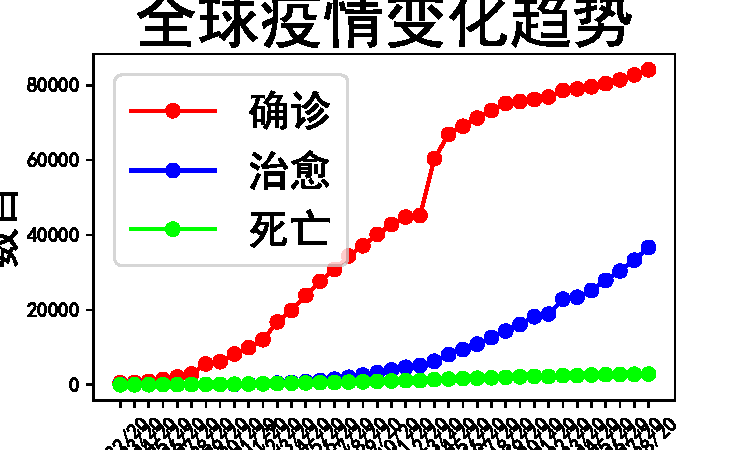
\includegraphics[height=0.5\textwidth]{d:/github_repo/wmy-python-homework/epidemic_analysis/epidemic_analysis_files/figure-latex/unnamed-chunk-6-1} \end{center}

\begin{figure}
\centering
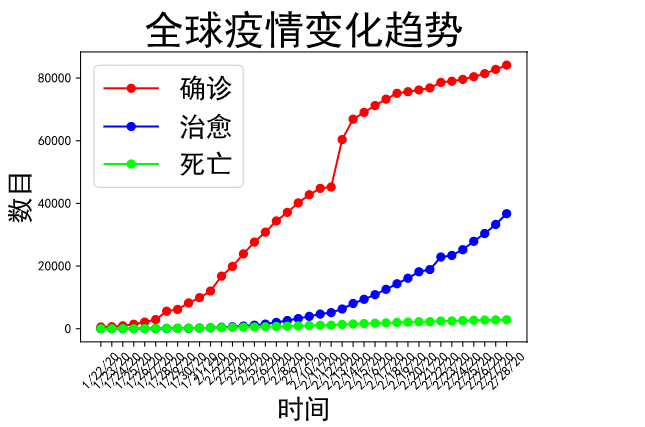
\includegraphics{./fig1.png}
\caption{fig1}
\end{figure}

\begin{lstlisting}[language=Python]

#下面看看新冠肺炎的死亡率,首先计算死亡率数据,然后就可以直接画图
death_rate = (all_deaths/all_confirmed)*100
plt.plot(death_rate,color = 'lime',label = '死亡',marker = 'o')
plt.xticks(rotation = 45,size = 10)
\end{lstlisting}

\begin{lstlisting}[language=Python]
plt.yticks(size = 15)
\end{lstlisting}

\begin{lstlisting}[language=Python]
plt.xlabel('时间',size = 20)
plt.ylabel('死亡率',size = 20)
plt.title('全球疫情死亡率',size =30)
\end{lstlisting}

\begin{center}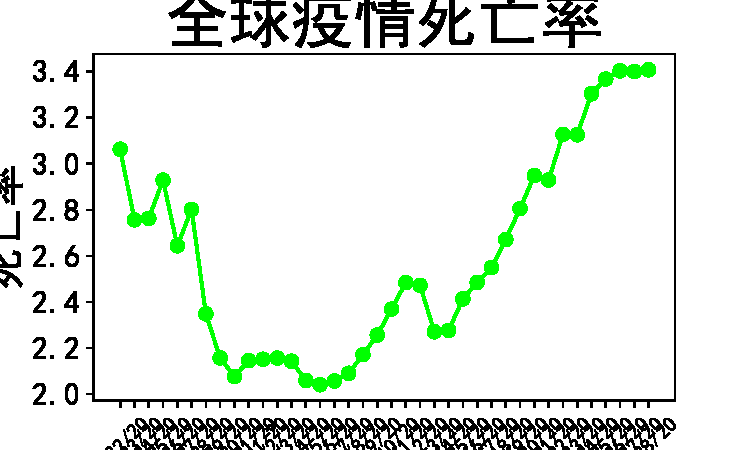
\includegraphics[height=0.5\textwidth]{d:/github_repo/wmy-python-homework/epidemic_analysis/epidemic_analysis_files/figure-latex/unnamed-chunk-7-1} \end{center}

\begin{figure}
\centering
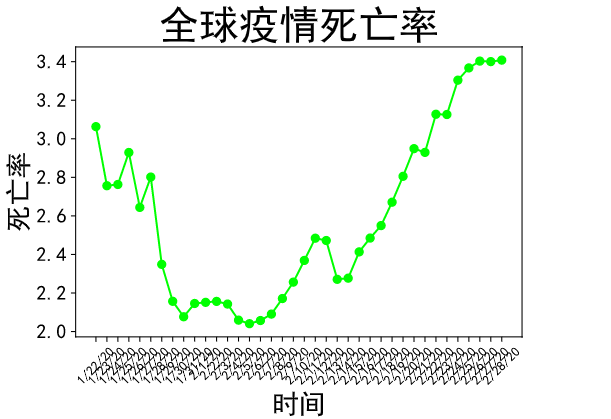
\includegraphics{./fig2.png}
\caption{fig2}
\end{figure}

\begin{lstlisting}[language=Python]

#由于本次疫情主要发生在中国大陆,下面来具体研究下中国大陆的疫情情况,首先从全部数据中提取出中国大陆的数据。里面包含了省份,以及每个省最新的确诊数,治愈数,死亡数。
last_update = '2/28/20' #设置最新数据日期
China_cases = confirmed[['Province/State',last_update]][confirmed['Country/Region']=='Mainland China']
China_cases['recovered'] = recovered[[last_update]][recovered['Country/Region']=='Mainland China']
China_cases['deaths'] = deaths[[last_update]][deaths['Country/Region']=='Mainland China']
China_cases = China_cases.set_index('Province/State')
China_cases = China_cases.rename(columns = {last_update:'confirmed'})
China_cases
\end{lstlisting}

\begin{figure}
\centering
\includegraphics{./表4.png}
\caption{表4}
\end{figure}

\begin{lstlisting}[language=Python]
#下面画出中国大陆每个省份的疫情数量图
Mianland_China = China_cases.sort_values(by='confirmed',ascending=True)
Mianland_China.plot(kind='barh',figsize=(20,30),color = ['red','blue','lime'],width = 1,rot = 2)
plt.title('中国大陆各省市疫情数量',size = 30)
plt.xlabel('省/市',size = 20)
plt.ylabel('数量',size = 20)
plt.xticks(size = 15)
\end{lstlisting}

\begin{lstlisting}[language=Python]
plt.yticks(size = 20)
\end{lstlisting}

\begin{lstlisting}[language=Python]
plt.legend(bbox_to_anchor = (0.95,0.95),fontsize = 20)
#可以看到,湖北省三项数据高居第一位,且远远高于其他省份。
\end{lstlisting}

\begin{center}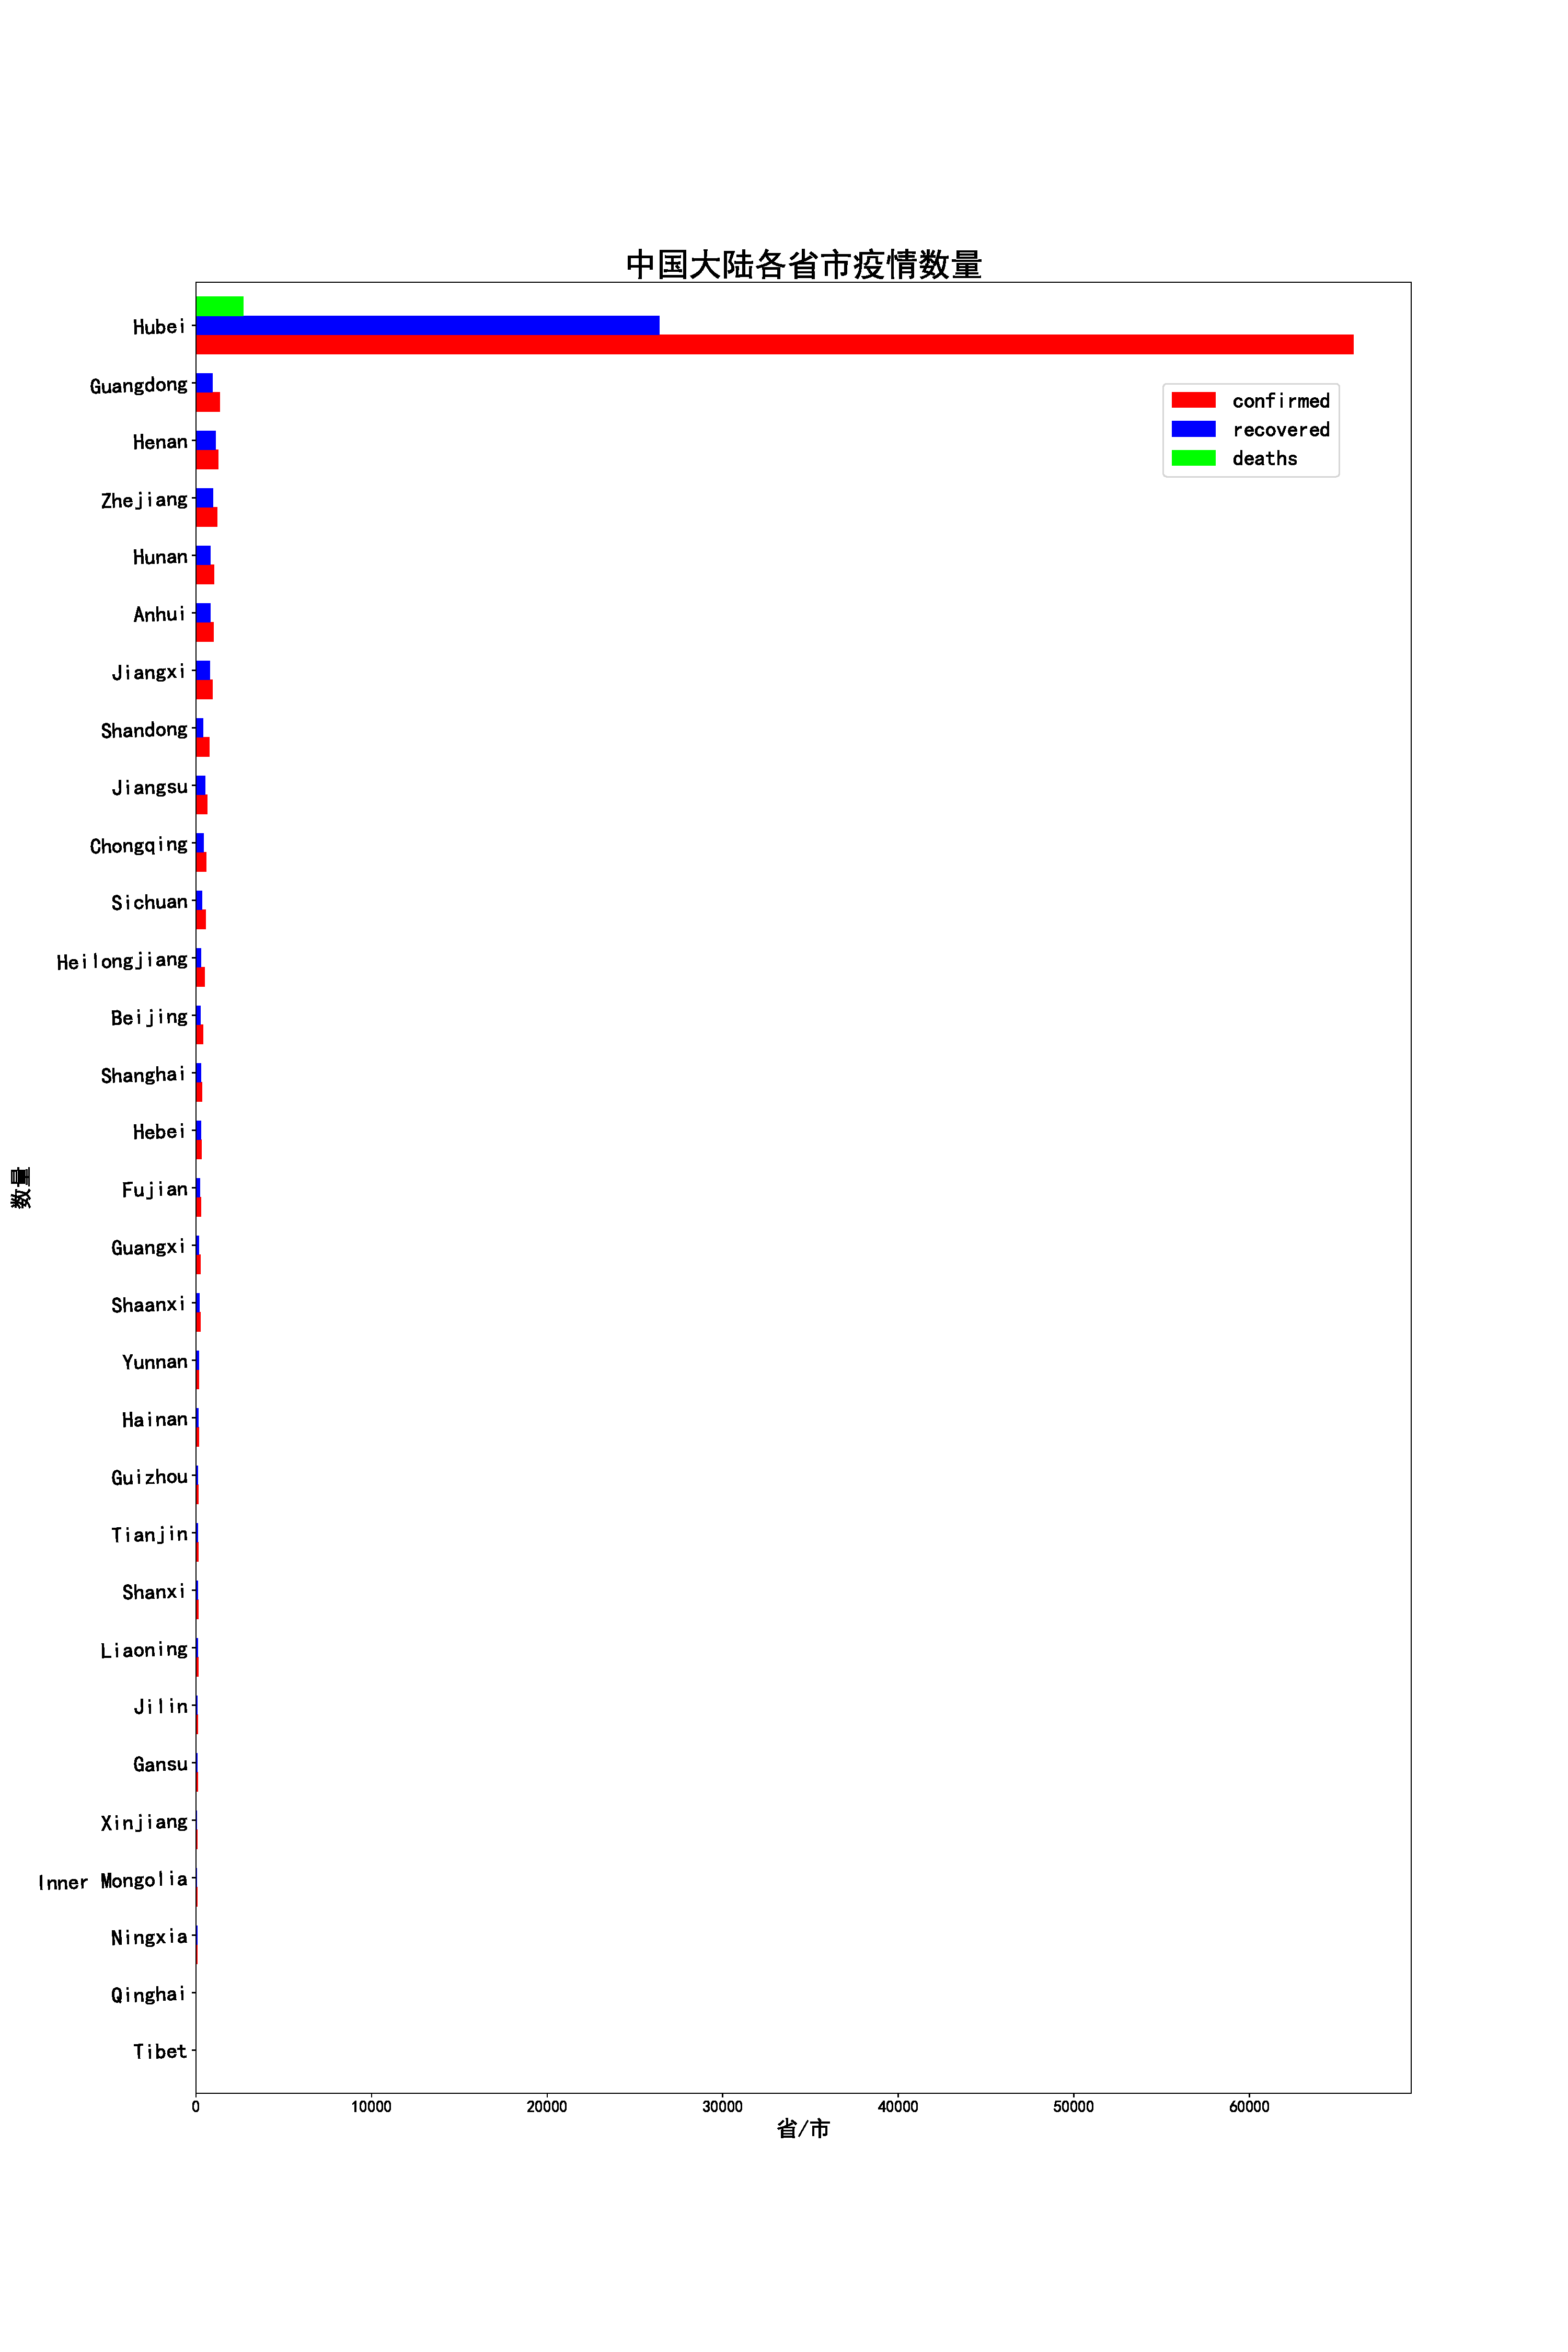
\includegraphics[height=0.5\textwidth]{d:/github_repo/wmy-python-homework/epidemic_analysis/epidemic_analysis_files/figure-latex/unnamed-chunk-9-1} \end{center}

\begin{figure}
\centering
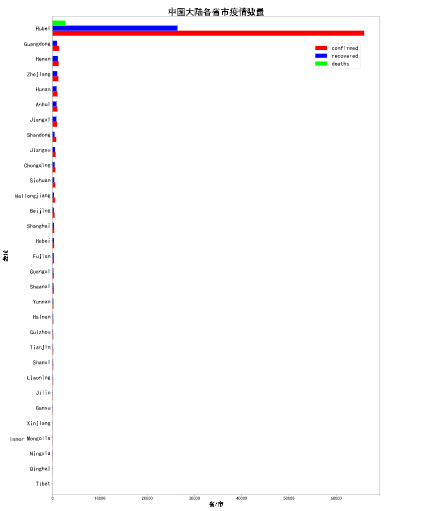
\includegraphics{./fig3.png}
\caption{fig3}
\end{figure}

\begin{lstlisting}[language=Python]
#下面看看中国大陆的治愈率和死亡率数据,数据使用下面的代码即可计算出来,最终结果在recover_rate和death_rate里。
confirmed_China = confirmed[confirmed['Country/Region']=='Mainland China']
confirmed_China = np.sum(confirmed_China.iloc[:,4:])
recovered_China = recovered[recovered['Country/Region']=='Mainland China']
recovered_China = np.sum(recovered_China.iloc[:,4:])
deaths_China = deaths[deaths['Country/Region']=='Mainland China']
deaths_China = np.sum(deaths_China.iloc[:,4:])
recover_rate = (recovered_China/confirmed_China)*100  #中国地区的治愈率
deaths_rate = (deaths_China/confirmed_China)*100#中国各地区的死亡率
#接下来画图
plt.plot(recover_rate,color = 'blue',label = '治愈率',marker = 'o')
plt.plot(deaths_rate,color = 'lime',label = '死亡率',marker = 'o')
plt.title('中国大陆治愈率 VS 死亡率')
plt.xlabel('时间',size = 20)
plt.ylabel('数量',size = 20)
plt.xticks(rotation = 45,size = 10)
\end{lstlisting}

\begin{lstlisting}[language=Python]
plt.yticks(size =15)
\end{lstlisting}

\begin{lstlisting}[language=Python]
plt.legend(loc = 'upper left',fontsize = 20)
#虽然在1月25日-1月31日期间死亡率略高于治愈率,但其他时间段,治愈率远远高于死亡率
\end{lstlisting}

\begin{center}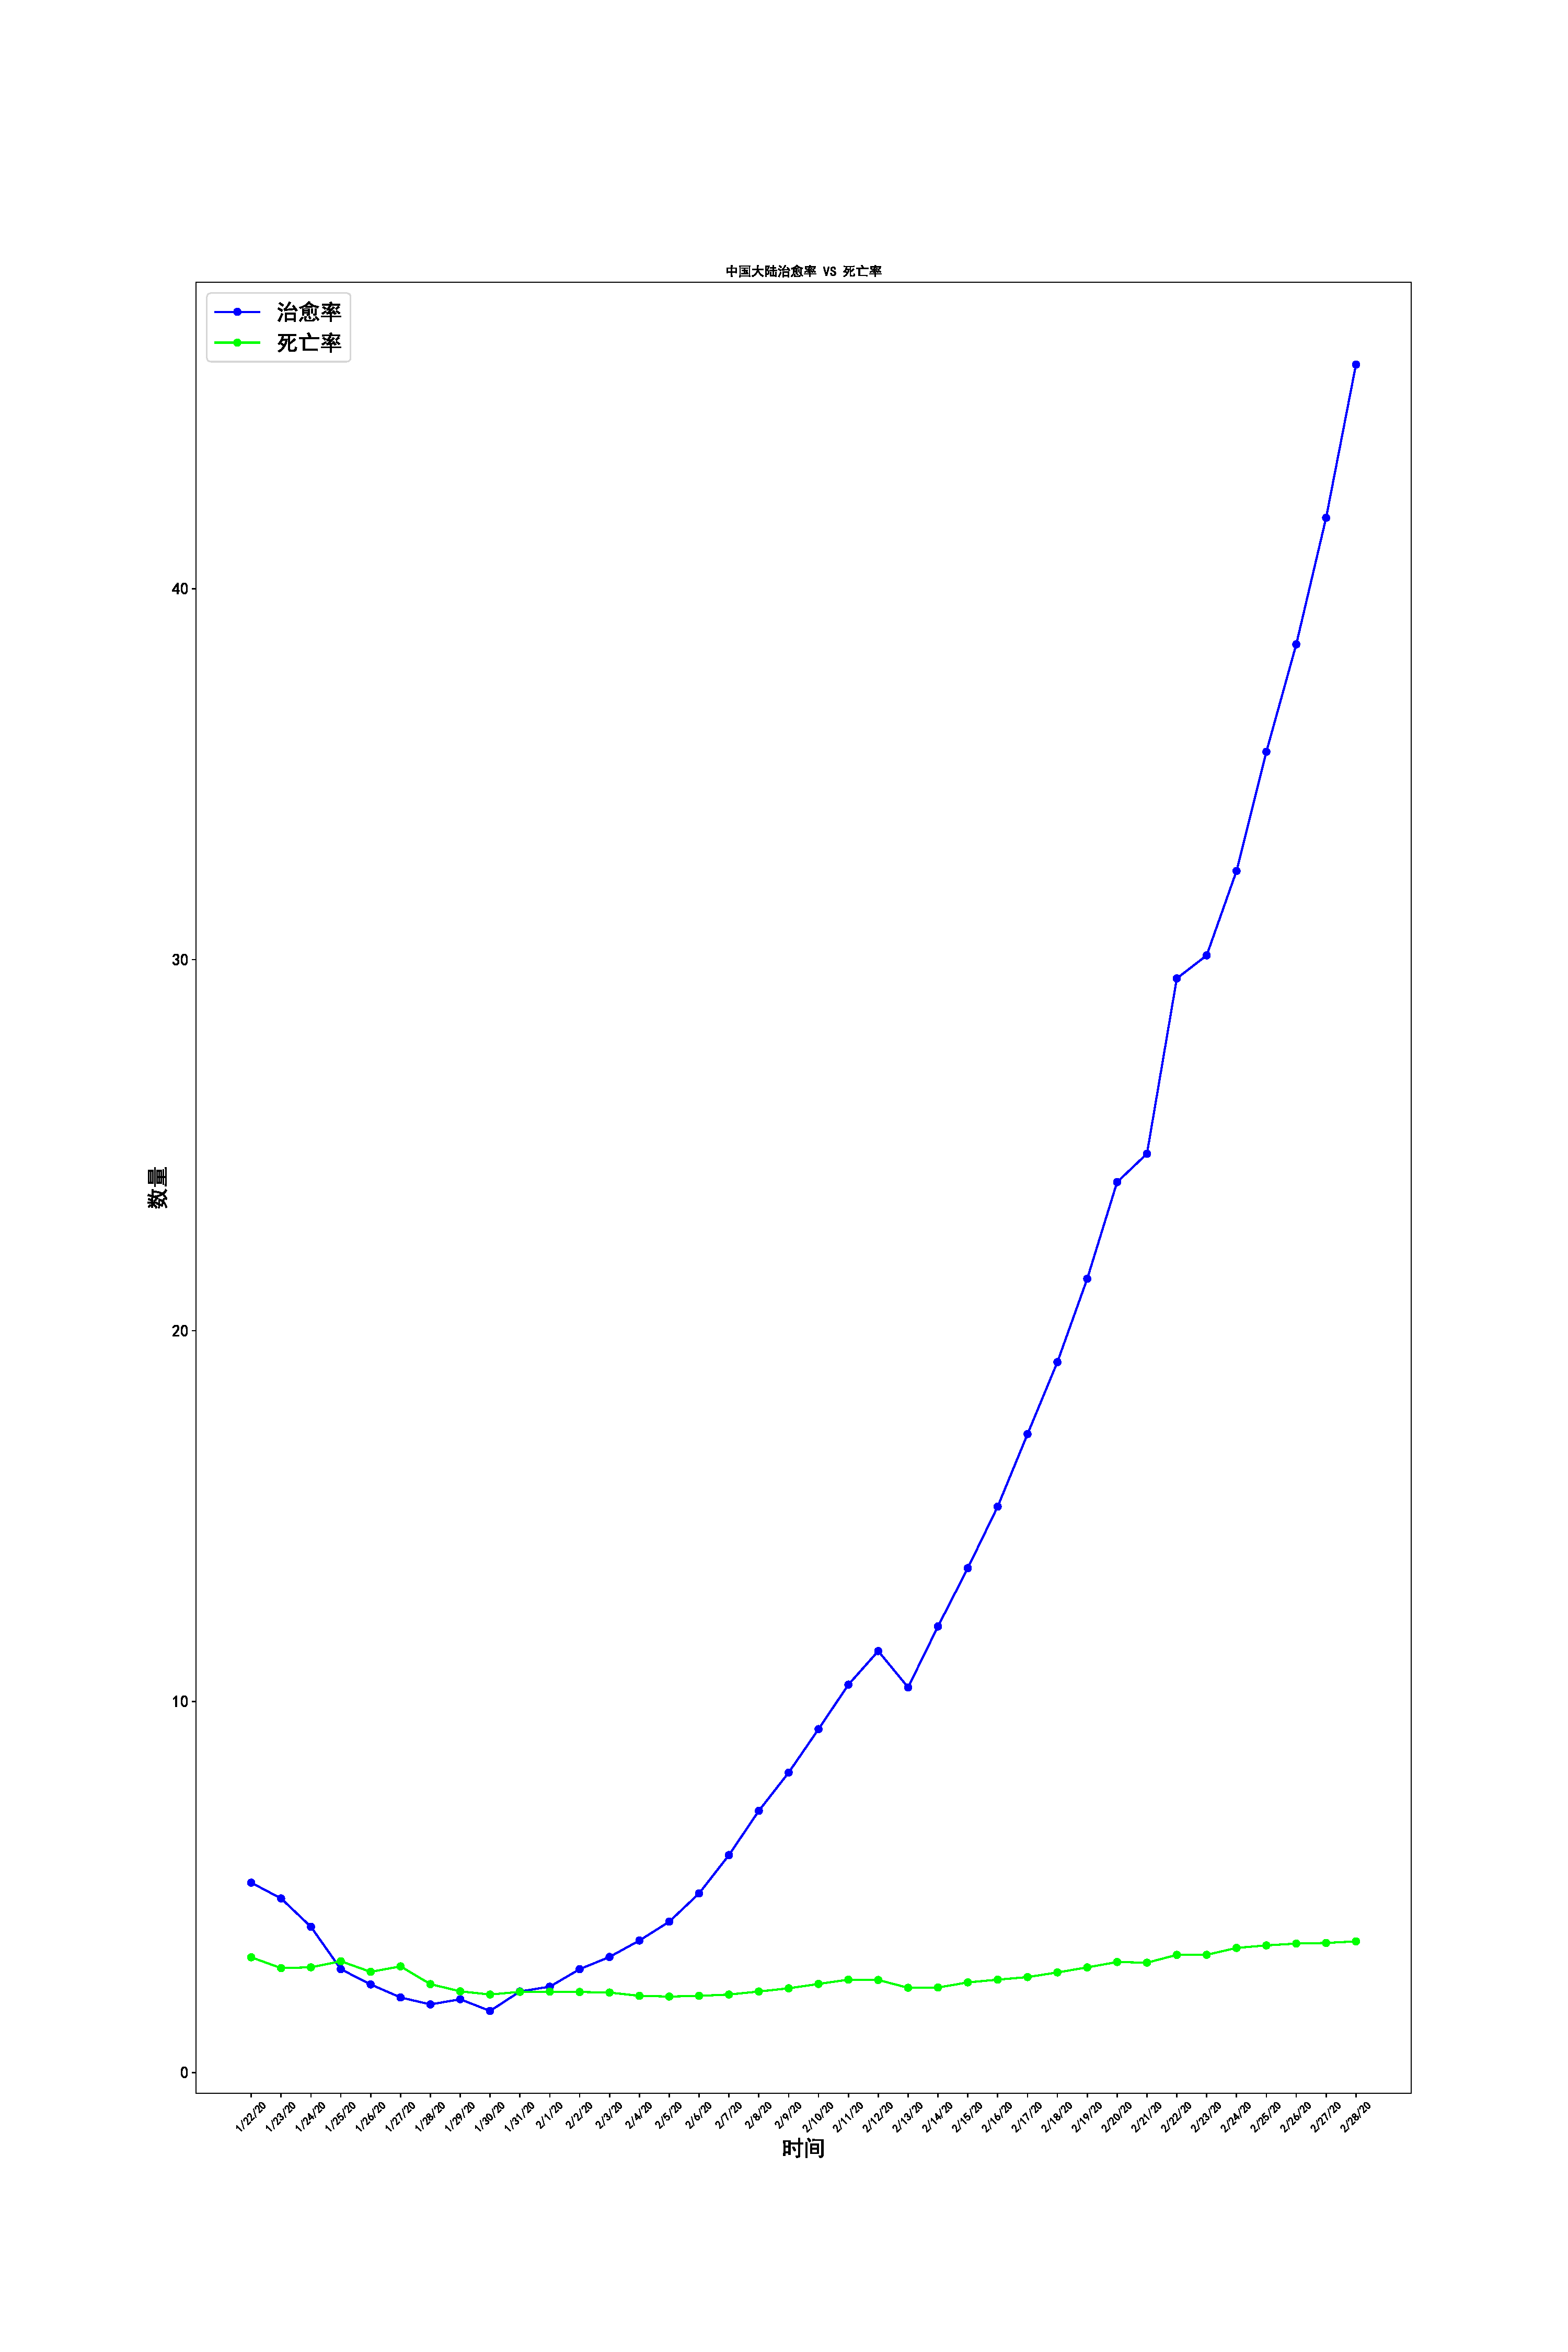
\includegraphics[height=0.5\textwidth]{d:/github_repo/wmy-python-homework/epidemic_analysis/epidemic_analysis_files/figure-latex/unnamed-chunk-10-1} \end{center}

\begin{figure}
\centering
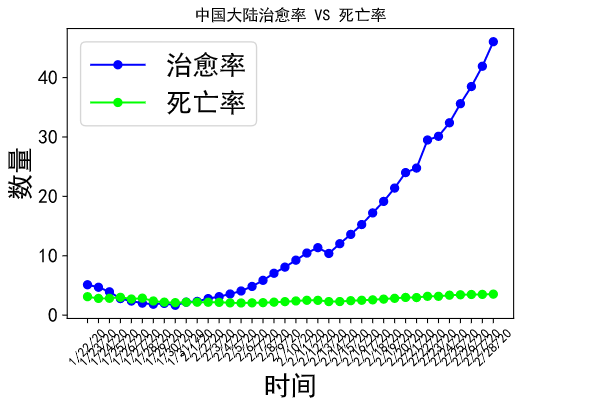
\includegraphics{./fig4.png}
\caption{fig4}
\end{figure}

\begin{lstlisting}[language=Python]
#那中国大陆其他地区这一情况咋样呢?代码大同小异,我们一起来看看,首先还是提取出其他地区的数据。
confirmed_others = confirmed[confirmed['Country/Region'] != 'Mainland China']
confirmed_others = np.sum(confirmed_others.iloc[:,4:])
recovered_others = recovered[recovered['Country/Region'] != 'Mainland China']
recovered_others = np.sum(recovered_others.iloc[:,4:])
deaths_others = deaths[deaths['Country/Region']!='Mainland China']
deaths_others = np.sum(deaths_others.iloc[:,4:])
recover_rate_others = (recovered_others/confirmed_others)*100  #其他地区的治愈率
deaths_rate_others = (deaths_others/confirmed_others)*100#其他各地区的死亡率
#接下来画图
plt.plot(recover_rate_others,color = 'blue',label = '治愈率',marker = 'o')
plt.plot(deaths_rate_others,color = 'lime',label = '死亡率',marker = 'o')
plt.title('其他地区治愈率 VS 死亡率',size = 30)
plt.xlabel('时间',size = 20)
plt.ylabel('数量',size = 20)
plt.xticks(rotation = 45,size = 10)
\end{lstlisting}

\begin{lstlisting}[language=Python]
plt.yticks(size =15)
\end{lstlisting}

\begin{lstlisting}[language=Python]
plt.legend(loc = 'upper left',fontsize = 20)
\end{lstlisting}

\begin{center}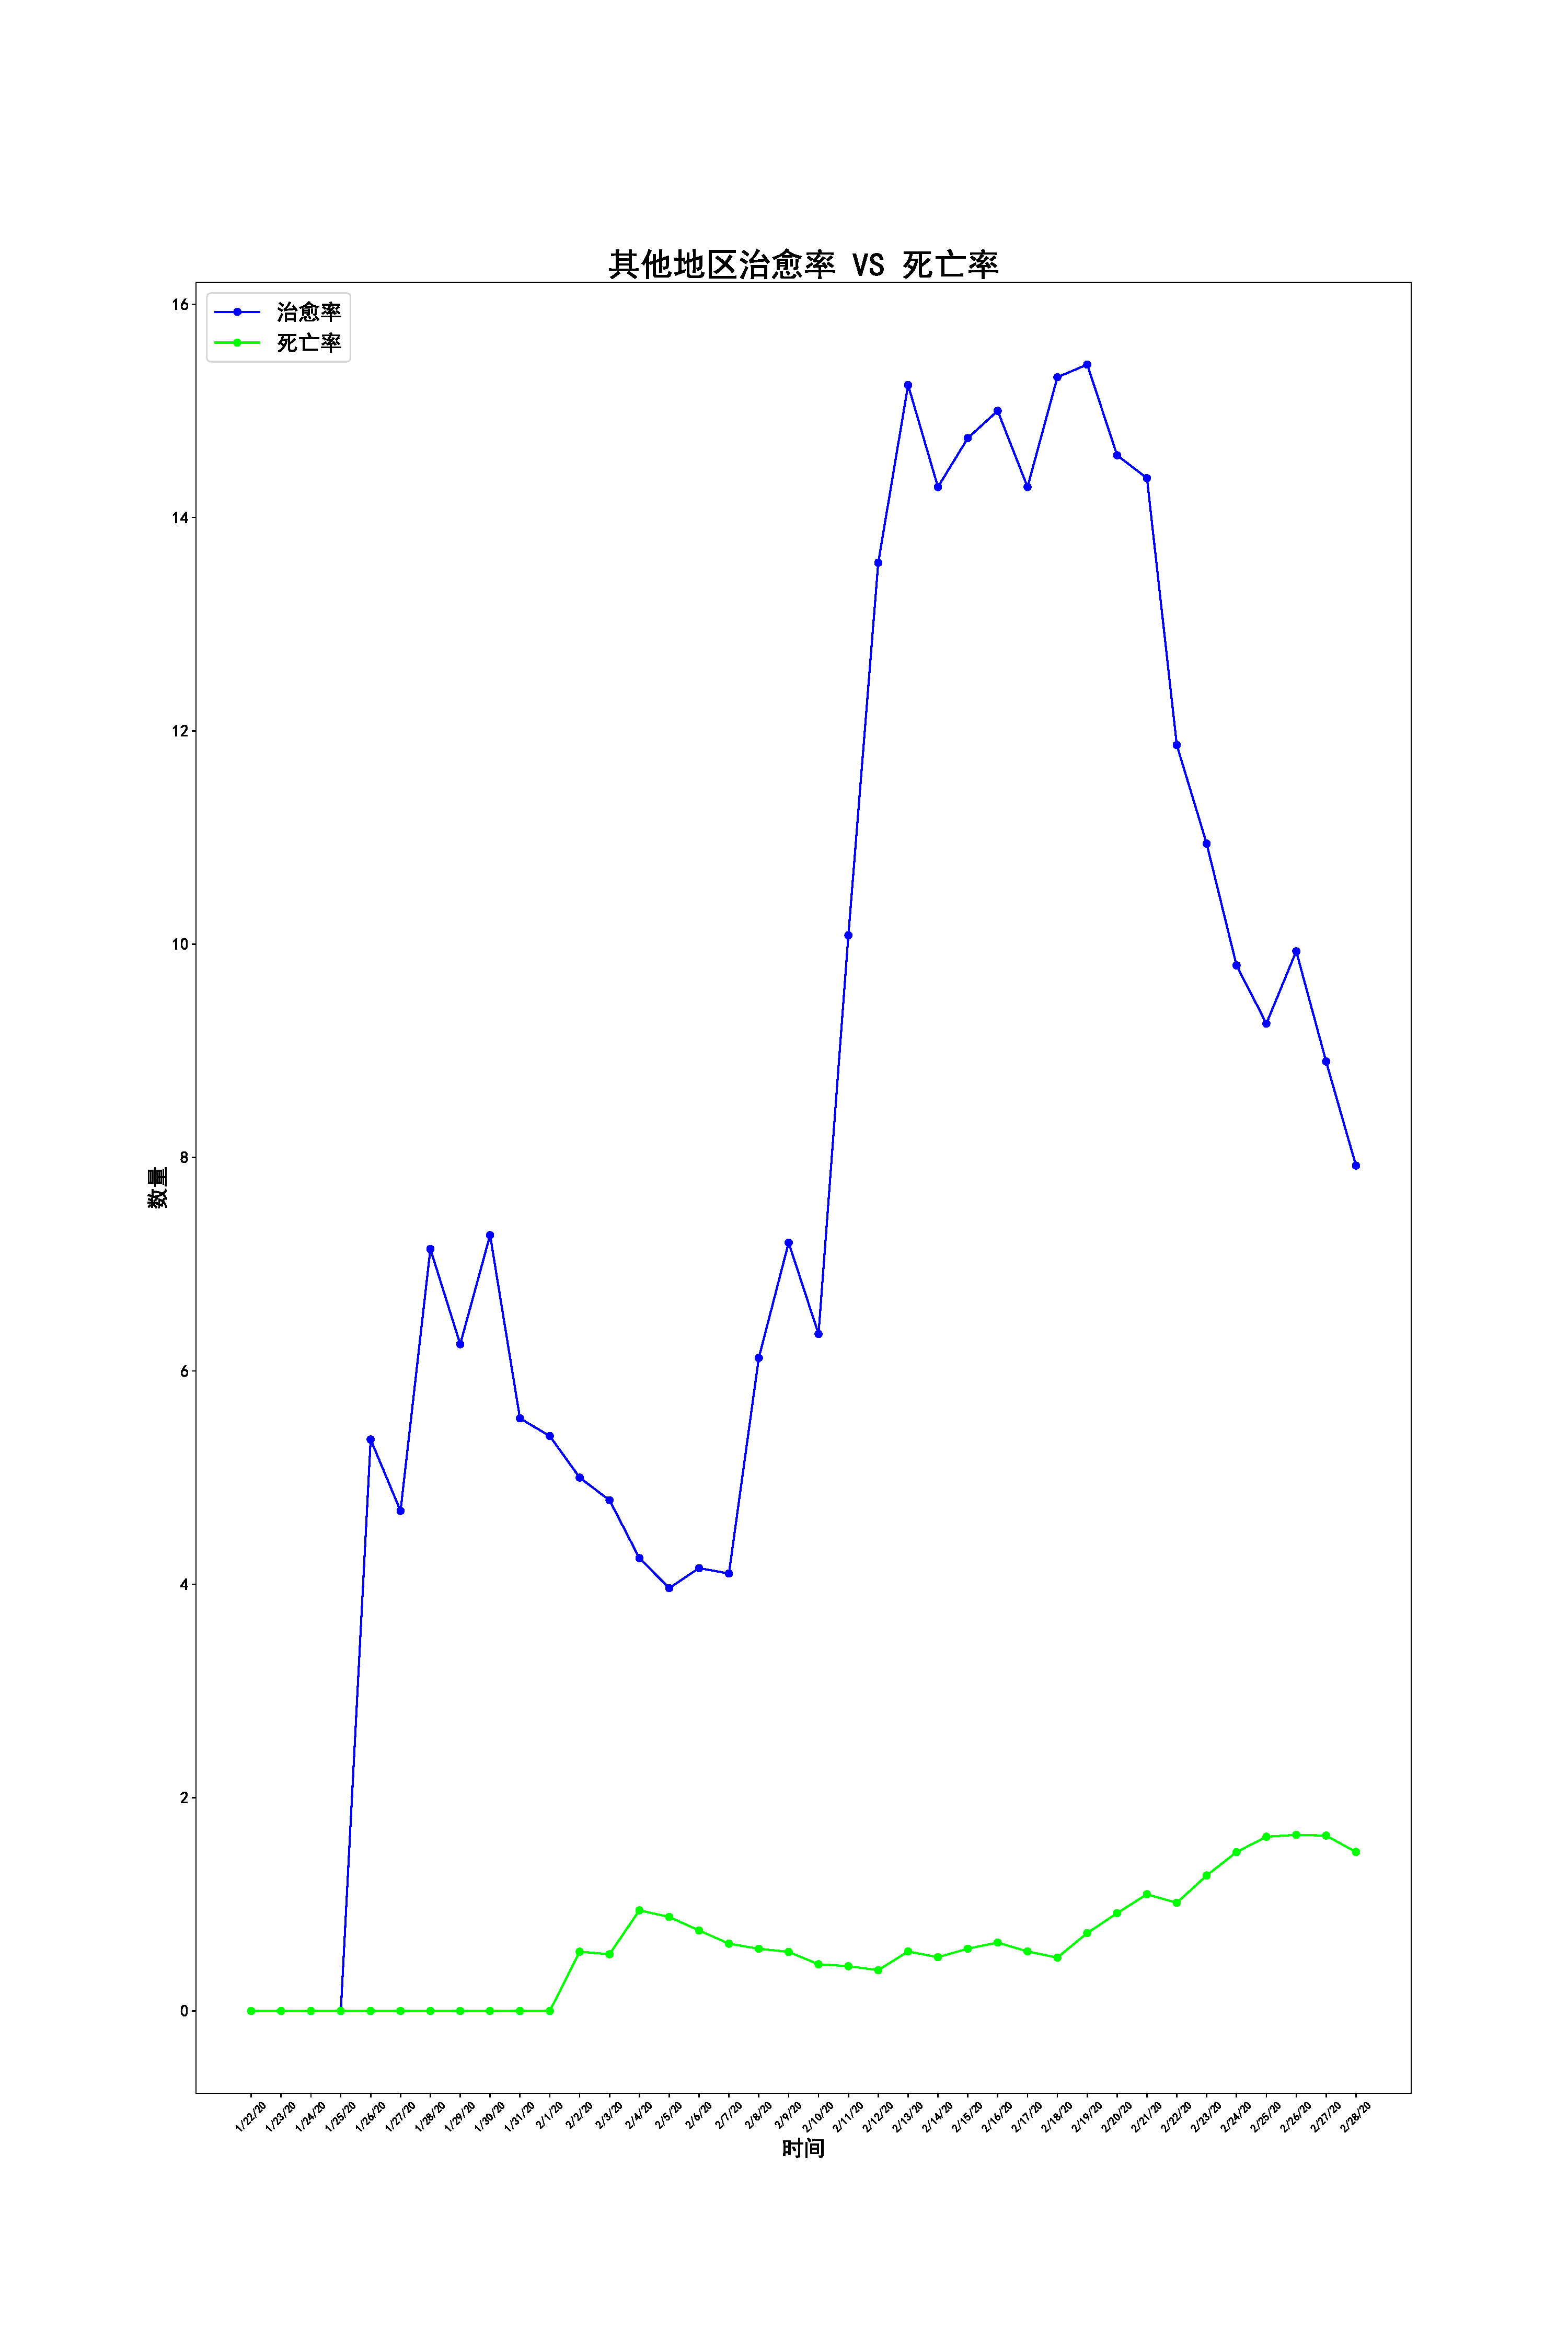
\includegraphics[height=0.5\textwidth]{d:/github_repo/wmy-python-homework/epidemic_analysis/epidemic_analysis_files/figure-latex/unnamed-chunk-11-1} \end{center}

\begin{figure}
\centering
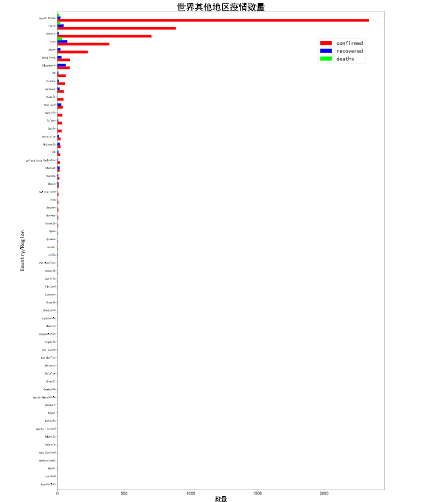
\includegraphics{./fig6.png}
\caption{fig5}
\end{figure}

\begin{lstlisting}[language=Python]
#接下来看看其他地区疫情数量。首先还是提出其他地区的数据
others = confirmed[['Country/Region',last_update]][confirmed['Country/Region'] != 'Mainland China']
others['recovered'] = recovered[[last_update]][recovered['Country/Region'] != 'Mainland China']
others['deaths'] = deaths[[last_update]][deaths['Country/Region'] != 'Mainland China']

others_countries = others.rename(columns = {last_update:'confirmed'})
others_countries = others_countries.set_index('Country/Region')
others_countries = others_countries.groupby('Country/Region').sum()
#接着画图
others_countries.sort_values(by = 'confirmed',ascending = True).plot(kind='barh',figsize=(20,30),color = ['red','blue','lime'], width=1,rot=2)
plt.title('世界其他地区疫情数量', size=30)
plt.ylabel('Country/Region',size = 20)
plt.xlabel('数量',size = 20)
plt.yticks(size=10)
\end{lstlisting}

\begin{lstlisting}[language=Python]
plt.xticks(size=15)
\end{lstlisting}

\begin{lstlisting}[language=Python]
plt.legend(bbox_to_anchor=(0.95,0.95),fontsize = 20)
plt.show()
#从图可以看到,韩国,意大利,日本这些地区也有很多新冠肺炎患者。
\end{lstlisting}

\begin{center}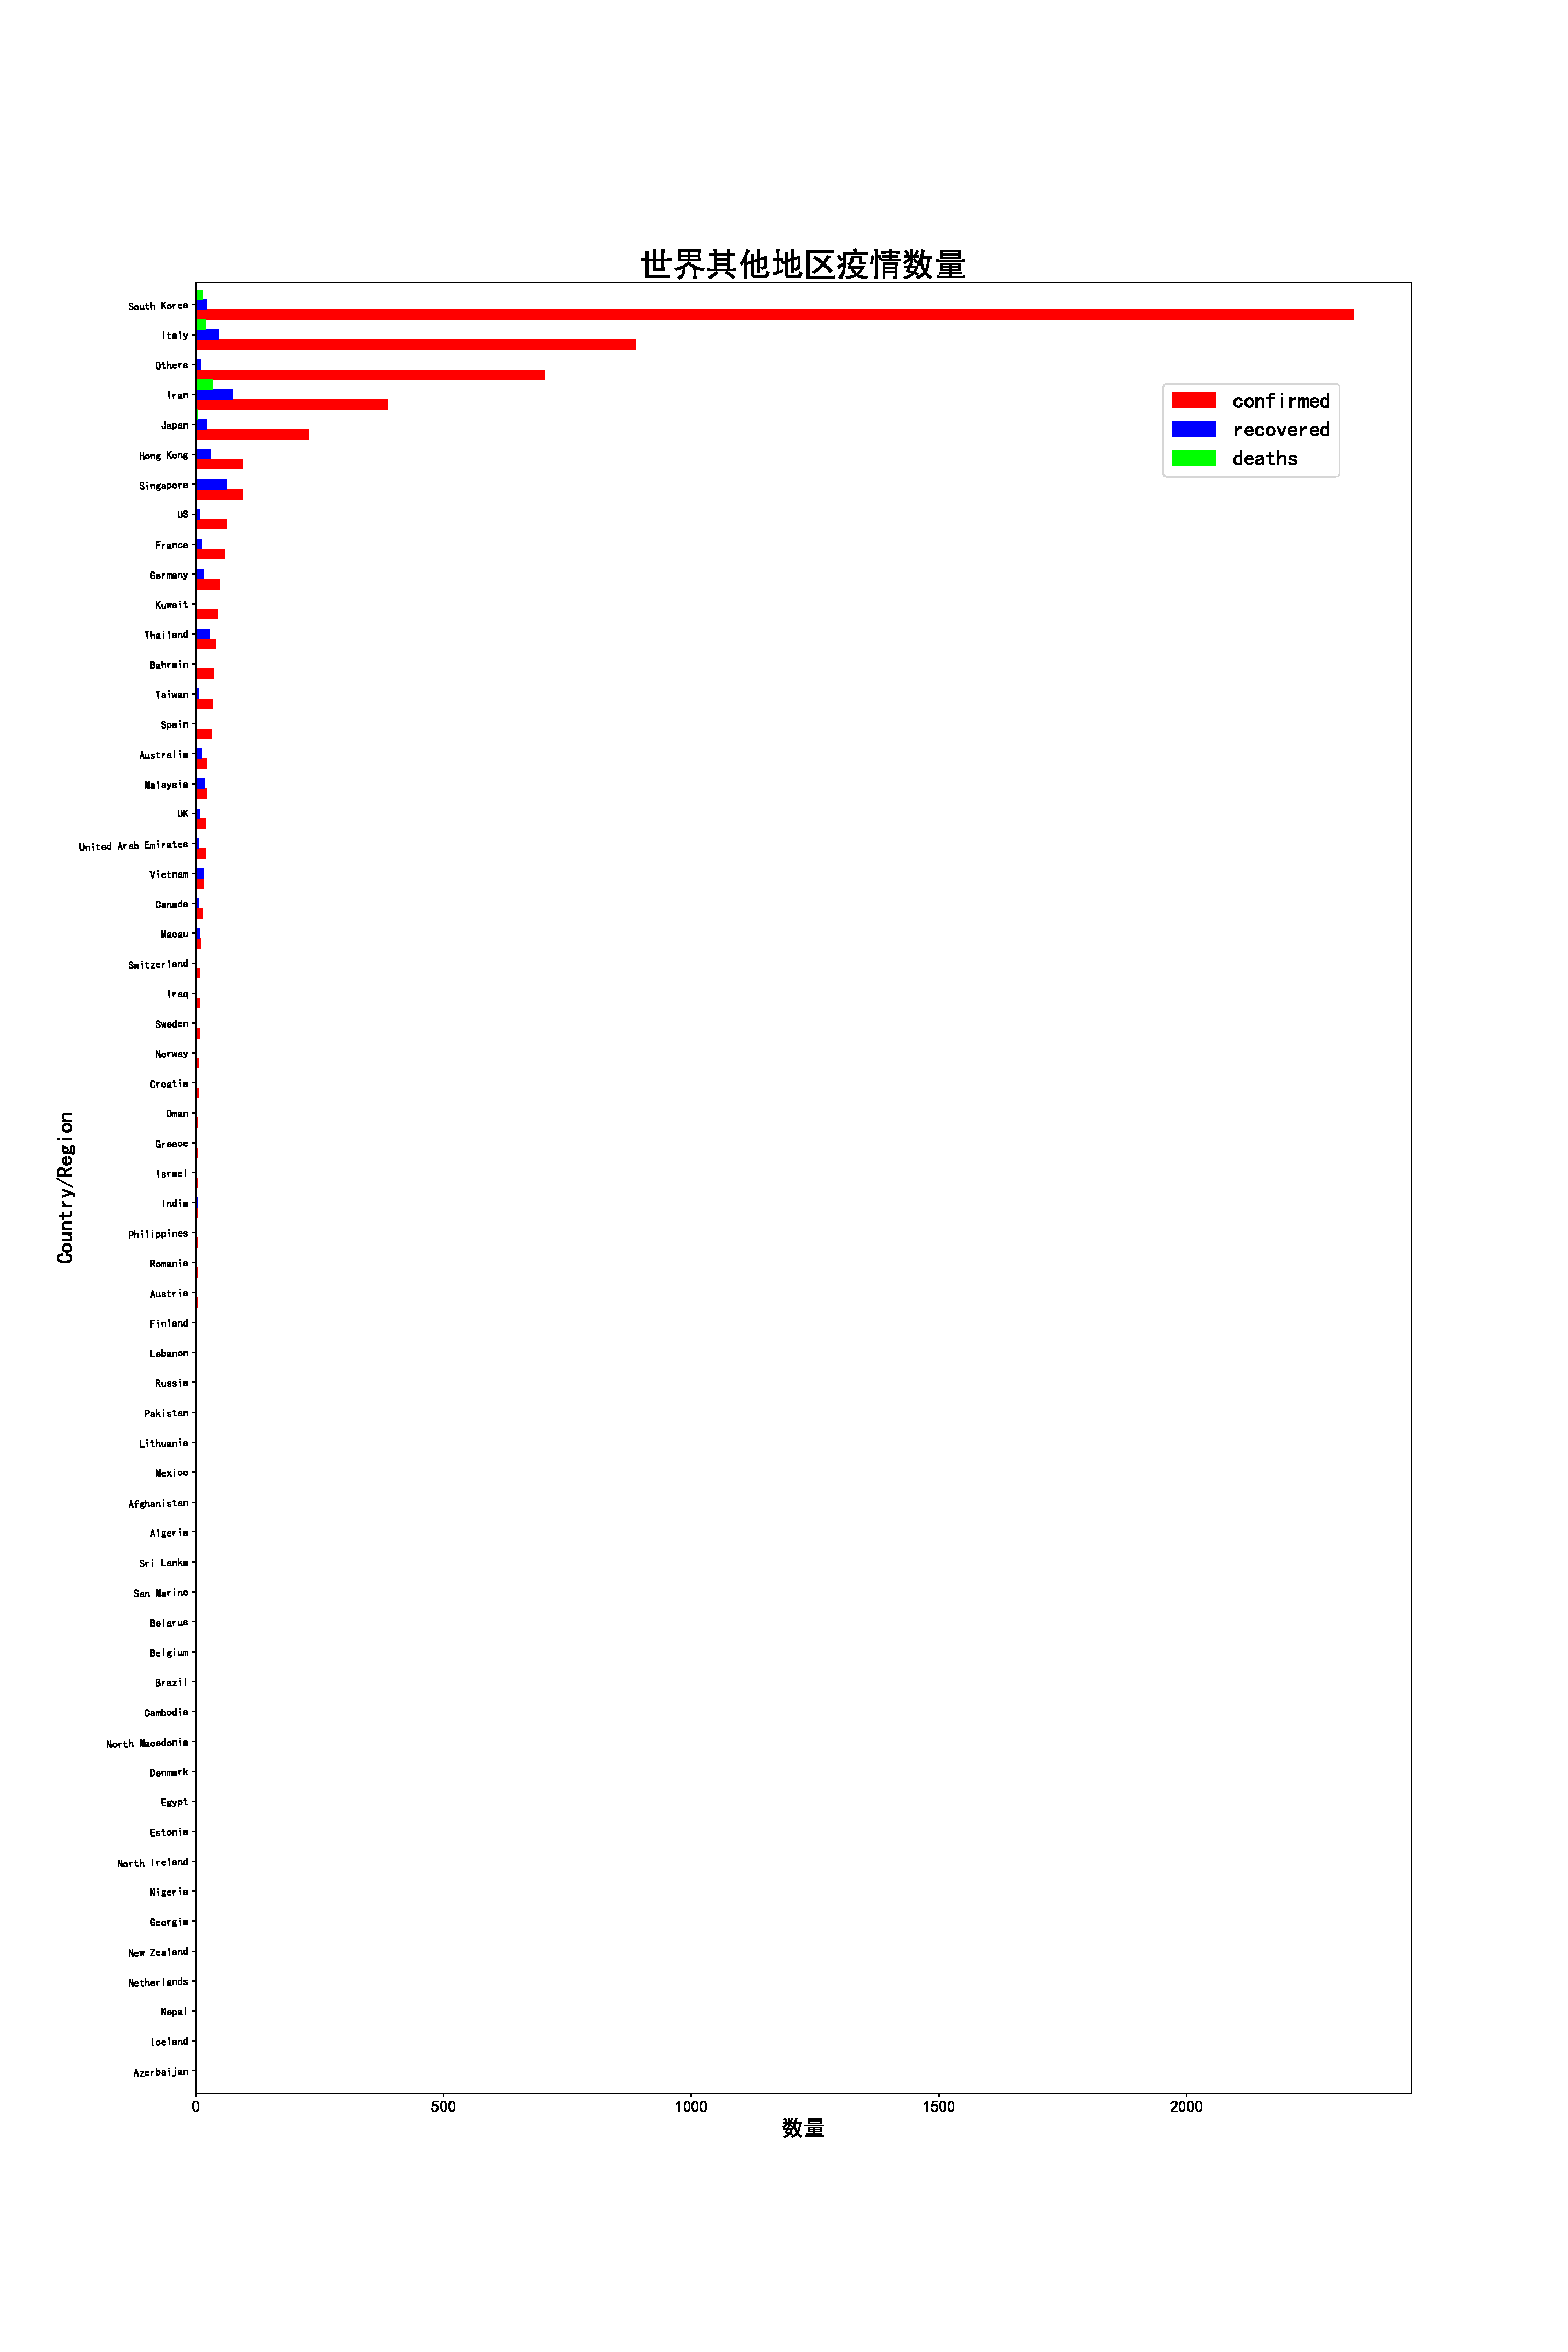
\includegraphics[height=0.5\textwidth]{d:/github_repo/wmy-python-homework/epidemic_analysis/epidemic_analysis_files/figure-latex/unnamed-chunk-12-1} \end{center}

\begin{figure}
\centering
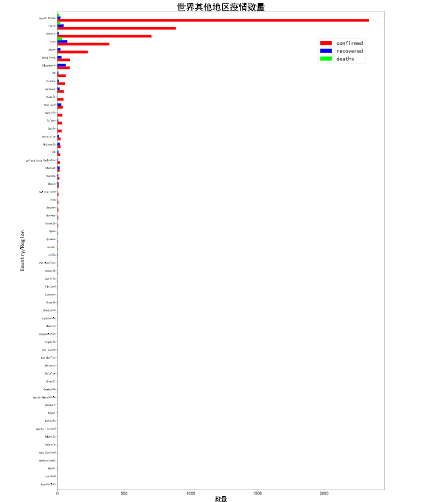
\includegraphics{./fig6.png}
\caption{fig6}
\end{figure}

\section{绘制疫情地图}

这里主要用到两个python包,一个是folium包,这个包也是笔者最近才发现的绘图包,类似于R语言绘图里的ggplot2,可以添加图层来定义一个Map对象,最后以几种方式将Map对象展现出来。这里有一个详细教程,感兴趣的可以看看https://python-visualization.github.io/folium/。另一个包就是plotly了,这也是一个强大的绘图包,详细教程请看这里https://plot.ly/python/plotly-express/。

首先是folium包绘制地图,import folium,只需要导入包就可以了,没下载这个包的记得下载才能使用。我们在前面数据里加入中国大陆的数据,并使用武汉的经纬度。

\begin{lstlisting}[language=Python]
import folium
others = confirmed[['Country/Region','Lat','Long',last_update]][confirmed['Country/Region'] != 'Mainland China']
others['recovered'] = recovered[[last_update]][recovered['Country/Region'] != 'Mainland China']
others['death'] = deaths[[last_update]][deaths['Country/Region'] != 'Mainland China']
others_countries = others.rename(columns = {last_update:'confirmed'})
\end{lstlisting}

\begin{figure}
\centering
\includegraphics{./表5.png}
\caption{表5}
\end{figure}

\begin{lstlisting}[language=Python]
#然后开始正式构建地图
#定义一个world_map对象;location的格式为[纬度,经度];zoom_start表示初始地图的缩放尺寸,数值越大放大程度越大;tiles为地图类型,用于控制绘图调用的地图样式,默认为'OpenStreetMap',也有一些其他的内建地图样式,如'Stamen  Terrain'、'Stamen Toner'、'Mapbox Bright'、'Mapbox Control Room'等;也可以传入'None'来绘制一个没有风格的朴素地图,或传入一个URL来使用其它的自选osm。
#然后往world_map里添加其他元素,注意这里的for循环和最后的add_to是把经纬度点的信息一个一个的加进去
world_map = folium.Map(location=[10,-20],zoom_start=2.3,tiles='Stamen Toner')

for lat, lon, value, name in zip(others_countries['Lat'],others_countries['Long'],others_countries['confirmed'],others_countries['Country/Region']):
  folium.CircleMarker([lat, lon],
                              radius=10,
                              popup = ('<strong>Country</strong>: ' + str(name).capitalize()+'<br>' '<strong>Confirmed Cases</strong>: ' + str(value) + '<br>'),
                              color = "red",
                              fill_color = "red",
                              fill_opacity = 0.7).add_to(world_map)
\end{lstlisting}

\begin{lstlisting}[language=Python]
world_map
\end{lstlisting}

\begin{figure}
\centering
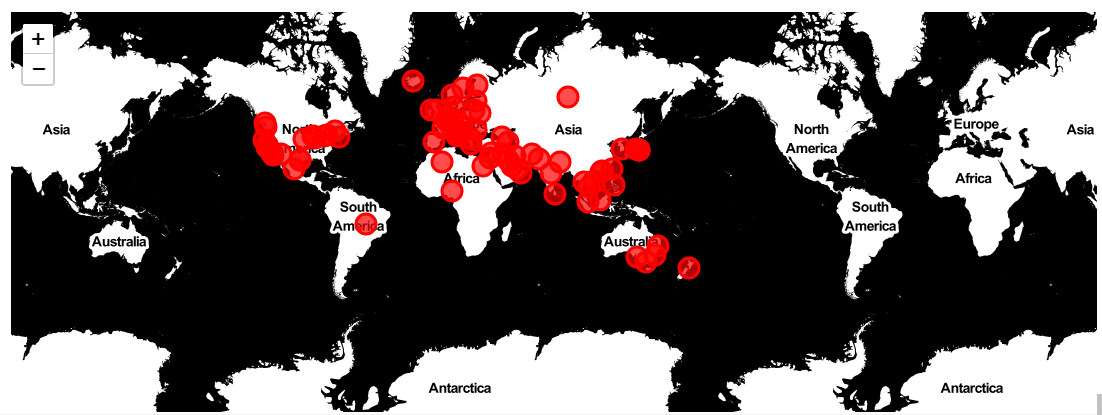
\includegraphics{./world_map.png}
\caption{world\_map}
\end{figure}

用plotly绘制每日疫情扩散地图

\begin{lstlisting}[language=Python]
import plotly.express as px
confirmed = confirmed.melt(id_vars = ['Province/State', 'Country/Region', 'Lat', 'Long'], var_name='date',value_name = 'confirmed')
confirmed
\end{lstlisting}

\begin{figure}
\centering
\includegraphics{./表6.png}
\caption{表6}
\end{figure}

\begin{lstlisting}[language=Python]
#date列转换成datetime格式的数据
confirmed['date_dt'] = pd.to_datetime(confirmed.date,format='%m/%d/%y')
confirmed.date = confirmed.date_dt.dt.date
confirmed.rename(columns={'Country/Region':'country','Province/State':'province'},inplace=True)
confirmed
\end{lstlisting}

\begin{figure}
\centering
\includegraphics{./表7.png}
\caption{表7}
\end{figure}

\begin{lstlisting}[language=Python]
#治愈数据
recovered = recovered.melt(id_vars = ['Province/State', 'Country/Region', 'Lat', 'Long'], var_name='date',value_name = 'recovered')
recovered['date_dt'] = pd.to_datetime(recovered.date, format="%m/%d/%y")
recovered.date = recovered.date_dt.dt.date
recovered.rename(columns={'Country/Region': 'country', 'Province/State': 'province'}, inplace=True)
#死亡数据
deaths = deaths.melt(id_vars = ['Province/State', 'Country/Region', 'Lat', 'Long'], var_name='date', value_name = 'deaths')
deaths['date_dt'] = pd.to_datetime(deaths.date, format="%m/%d/%y")
deaths.date = deaths.date_dt.dt.date
deaths.rename(columns={'Country/Region': 'country', 'Province/State': 'province'}, inplace=True)

merge_on = ['province', 'country', 'date']
all_data = confirmed.merge(deaths[merge_on + ['deaths']], how='left', on=merge_on).\
  merge(recovered[merge_on + ['recovered']], how='left', on=merge_on)
all_data
\end{lstlisting}

\begin{figure}
\centering
\includegraphics{./表8.png}
\caption{表8}
\end{figure}

\begin{lstlisting}[language=Python]
Coronavirus_map = all_data.groupby(['date_dt', 'province'])['confirmed', 'deaths','recovered', 'Lat', 'Long'].max().reset_index()
Coronavirus_map['size'] = Coronavirus_map.confirmed.pow(0.5)  # 创建实心圆大小
Coronavirus_map['date_dt'] = Coronavirus_map['date_dt'].dt.strftime('%Y-%m-%d')
\end{lstlisting}

\begin{figure}
\centering
\includegraphics{./表9.png}
\caption{表9}
\end{figure}

\begin{lstlisting}[language=Python]
fig = px.scatter_geo(Coronavirus_map, lat='Lat', lon='Long', scope='asia',
                     color="size", size='size', hover_name='province',
                     hover_data=['confirmed', 'deaths', 'recovered'],
                     projection="natural earth",animation_frame="date_dt",title='亚洲地区疫情扩散图')
fig.update(layout_coloraxis_showscale=False)
\end{lstlisting}

\begin{lstlisting}[language=Python]
fig.show()
\end{lstlisting}

\begin{figure}
\centering
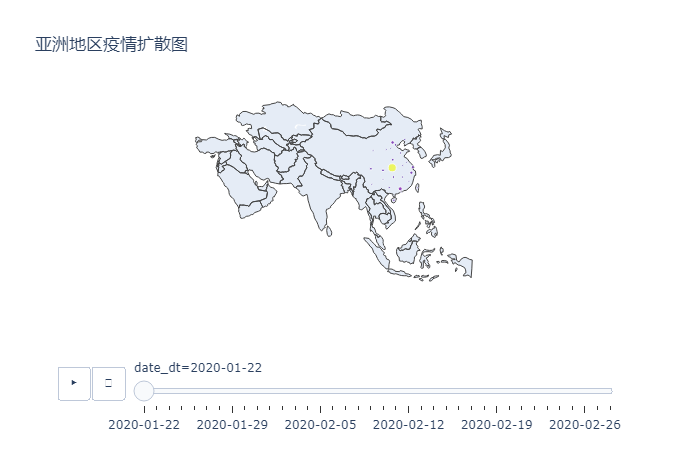
\includegraphics{./fig7.png}
\caption{fig7}
\end{figure}


\end{document}
